\documentclass[11pt,a4paper,twoside]{tesis}
% SI NO PENSAS IMPRIMIRLO EN FORMATO LIBRO PODES USAR
%\documentclass[11pt,a4paper]{tesis}

\usepackage{graphicx}
\usepackage[utf8]{inputenc}
\usepackage[spanish]{babel}
\usepackage[left=3cm,right=3cm,bottom=3.5cm,top=3.5cm]{geometry}
\usepackage{natbib}
\usepackage{hyperref}
\bibliographystyle{abbrvnat}

\begin{document}

%%%% CARATULA

\def\autor{Juan Manuel Pérez}
\def\tituloTesis{Título de tesis: \vspace{.2cm} \\ Técnicas y alcances}
\def\runtitulo{Título de tesis: \vspace{.2cm} \\ Técnicas y alcances}
\def\runtitle{Star Wars: Rebellion and Empire}
\def\director{Franco Luque}
\def\codirector{Agustín Gravano}
\def\lugar{Buenos Aires, 2021}
\newcommand{\HRule}{\rule{\linewidth}{0.2mm}}
%
\thispagestyle{empty}

\begin{center}\leavevmode

    \vspace{-2cm}

    \begin{tabular}{l}
        
\includegraphics[width=2.6cm]{img/logofcen.png}
    \end{tabular}


    {\large \sc Universidad de Buenos Aires

    Facultad de Ciencias Exactas y Naturales

    Departamento de Computaci\'on}

    \vspace{6.0cm}

    %\vspace{3.0cm}
    %{
    %\Large \color{red}
    %\begin{tabular}{|p{2cm}cp{2cm}|}
    %\hline
    %& Pre-Final Version: \today &\\
    %\hline
    %\end{tabular}
    %}
    %\vspace{2.5cm}

    \begin{huge}
        \textbf{\tituloTesis}
    \end{huge}

    \vspace{2cm}

    {\large Tesis presentada para el título de Doctor de la Universidad de Buenos Aires en
        el área de Ciencias de la Computaci\'on}

    \vspace{2cm}

    {\Large \autor}

\end{center}

\vfill

{\large

    \begin{tabular}{l l}
        \vspace{.3cm} Director:              & Dr. Franco Luque                    \\
        \vspace{.3cm} Director Asistente:    & Dr. Agustín Gravano                 \\
        \vspace{.3cm} Consejero de Estudios: & Dr. Diego Fernández Slezak          \\
        Lugar de Trabajo:                    & Departamento de Computación         \\
                                             & Facultad de Cs. Exactas y Naturales \\
        \vspace{1cm}                         & Universidad de Buenos Aires         \\
        Buenos Aires, 2022                   &                                     \\
    \end{tabular}

    \vspace{.2cm}



    \vspace{.2cm}


}

\newpage\thispagestyle{empty}


%%%% ABSTRACTS, AGRADECIMIENTOS Y DEDICATORIA
\frontmatter
\pagestyle{empty}
%\begin{center}
%\large \bf \runtitulo
%\end{center}
%\vspace{1cm}
\chapter*{\runtitulo}

{

    \setstretch{1.5}

\noindent El discurso discriminatorio (también conocido como discurso de odio) puede describirse como aquel discurso en clave de intenso aborrecimiento, denigración y enemistad que ataca a un individuo o un grupo de individuos por poseer –o aparentar poseer– cierta característica protegida por tratados internacionales como el sexo, el género, la etnia, etc. En los últimos años, este tipo de discurso ha tomado gran relevancia en redes sociales y otros medios virtuales debido a su intensidad y a su relación con actos violentos contra miembros de estos grupos. A raíz de esto, estados y organizaciones supranacionales como la Unión Europea han sancionado legislación que insta a las empresas de redes sociales a moderar y eliminar contenido discriminatorio, con particular foco en aquel que insta a la violencia física.

Debido a la enorme cantidad de contenido generado por usuarios en las redes sociales, es necesario contar con cierta automatización en esta tarea, bien para su análisis o para su moderación. Desde la óptica del procesamiento de lenguaje natural, la detección de discriminación puede entenderse como un problema de clasificación de texto: dado un texto generado por un usuario, predecir si es o no contenido discriminatorio. Así mismo, puede ser de interés predecir otras características: por ejemplo, si el texto contiene un llamado a la acción violenta, si está dirigido contra un individuo o un grupo, o el tipo de característica ofendida, entre otras.

Una de las limitaciones de los enfoques actuales para la detección del lenguaje discriminatorio es la falta de contexto en el mensaje. La mayoría de los estudios y recursos están hechos sobre datos fuera de contexto; es decir, mensajes aislados sin ningún tipo de contexto conversacional o del tema del cual se habla. Esto restringe la información disponible –tanto para un humano como para un sistema– para poder discernir si un texto social es discriminatorio. Otra información usualmente faltante es la característica atacada: es común que los datasets estén anotados de manera poco granular, no brindando información acerca de si la agresión es por motivos de sexo, género, clase social, etc. Por último, una limitación puntual del español es la poca disponibilidad de recursos para esta tarea.

En esta tesis pretendemos abordar algunas de las limitaciones marcadas. Por un lado, analizamos el impacto de agregar contexto a la detección de lenguaje discriminatorio en redes sociales. Para ello, construimos un conjunt de datos de tweets en base a las respuestas de los usuarios a los posteos de medios periodísticos en Twitter. Esto nos permite obtener dos tipos de contextos: uno “conversacional” al tener una respuesta a un tweet anterior, y otro más extenso al obtener el texto de la noticia en cuestión. El corpus fue recolectado sobre noticias relacionadas a la pandemia de COVID-19, en idioma español mayormente en su variedad dialectal rioplatense y anotado por hablantes nativos de ese dialecto con un nuevo modelo de etiquetado, que es granular respecto de las características ofendidas.

Sobre los comentarios de este dataset realizamos experimentos de detección de discurso de odio planteando dos tareas: detección binaria del lenguaje discriminatorio, donde sólo predecimos una etiqueta binaria indicando presencia de lenguaje discriminatorio; y detección granular, donde predecimos las características ofendidas. Usando técnicas del estado del arte, obtuvimos mejoras significativas en ambas tareas al agregar contexto como entrada de cada instancia, tanto en su forma corta (sólo el titular/tweet de la noticia) como en su forma larga (titular y cuerpo de la noticia). Así mismo, observamos que un clasificador entrenado para la tarea granular mejora levemente su performance al ser evaluado para la tarea binaria, obviando los posibles errores de motivos discriminatorios. Combinando la adición de contexto y granularidad, un clasificador para la detección de lenguaje discriminatorio obtiene mejoras considerables sobre un BERT en español que sólo consume el texto del comentario.

Considerando la detección de discurso de odio dentro del área más abarcativa de clasificación de documentos en dominios sociales, analizamos también algunos aspectos generales de tareas relacionadas como el análisis de sentimiento y la detección de emociones, entre otras. En particular, analizamos el desempeño de varias técnicas modernas de representación al ser entrenadas en dominios sociales. Comúnmente, los modelos de representación son entrenados a partir de textos de dominios formales, como pueden ser Wikipedia u otras fuentes similares. En esta tesis observamos que –desde los word embeddings hasta los modelos pre-entrenados basados en transformers– las representaciones generadas son robustas y mejoran la performance en un conjunto de tareas de clasificación en textos sociales. Sobre los modelos pre-entrenados, estudiamos el impacto de entrenarlos desde cero en textos sociales o efectuar una adaptación a este dominio.

Todos los estudios y recursos presentados en esta tesis fueron realizados en el idioma español. Como un objetivo secundario, pretendemos contribuir a mitigar la enorme asimetría de recursos existente en el área del procesamiento del lenguaje natural.


}


\bigskip

\noindent\textbf{Palabras claves:} Hate Speech, Natural Language Processing, Abusive Language Detection, Domain Adaptation, Social NLP.

\cleardoublepage
%\begin{center}
%\large \bf \runtitle
%\end{center}
%\vspace{1cm}
\chapter*{\runtitle}

\noindent
Hate speech can be described as speech containing intense hatred, denigration, and enmity that attacks an individual or a group of individuals because of possessing –or pretending to possess– any characteristic protected by international treaties such as gender, ethnicity, religion, language, among others. In recent years, this type of discourse has gained great relevance in social networks and other virtual media due to its intensity and its relationship with violent acts against members of these groups. As a result, states and supranational organizations –such as the European Union– have enacted legislation that urges social media companies to moderate and remove discriminatory content, with particular focus on that which promotes physical violence.

Due to the enormous amount of user-generated content on social media, it is necessary to have some degree of automation in this task, either for analysis or for moderation. From a natural language processing (NLP) perspective, hate speech detection can be understood as a text classification problem: given a text generated by a user, predict whether it is discriminatory content. Likewise, it may be of interest to predict other features: for example, if the text contains a call to violent action; if it is directed against an individual or a group; or the offended characteristic, among others.

One of the limitations of current approaches to hate speech detection is the lack of context. Most studies and resources are performed on data without context; that is, isolated messages without any type of conversational context or the topic being discussed. This restricts the information available –both for a human and for an automated system– to discern if a social text is hateful or not. Other information usually lacking is the offended characteristic: datasets are usually annotated with a low level of granularity, failing to provide information about whether the offending message attacks the individual or group due to their gender, social class, race, or whatsoever. Finally, a specific limitation of Spanish is the limited availability of resources for this task.

In this thesis, we intend to address some of the marked limitations. On the one hand, we analyze the impact of adding context to hate speech detection in social networks. To do this, we built a tweet dataset based on user responses to news media posts on Twitter. This provided us two types of contexts: a conversational context, given by the tweet and its answer, and another context given by the text of the news in question. This dataset was collected on news related to the COVID-19 pandemic, in the Spanish language in its Rioplatense dialectal variety. Native speakers of this dialect annotated the comments with a novel labeling model that is granular regarding the offended characteristics.

Using this dataset, we carried out hate speech detection experiments, proposing two tasks: "flat" detection of discriminatory language, where we only predict a binary label indicating the presence of discriminatory language; and "granular" detection, where we predict the attacked characteristics (n-binary classification tasks at the same time). Using state-of-the-art techniques, we obtained significant improvements in both tasks by adding context as input for each instance, both in its short form (only the headline/tweet of the news article) and in its long-form (headline and body of the news article). We also observed that a classifier trained for the "granular" task slightly improves its performance when being evaluated for the "flat" task, ignoring possible errors of discriminatory motives. Combining the addition of context and granularity, a classifier for the detection of discriminatory language obtained considerable improvements over a BERT in Spanish that only consumes the text of the comment.

Considering hate speech detection within the most comprehensive area of ​​document classification in social domains, we further explored  some general aspects of related tasks such as sentiment analysis and emotion detection, among others. In particular, we analyzed the performance of various modern representation techniques when trained in social domains. Commonly, NLP researchers train representation models on texts from "formal" domains, such as Wikipedia or other similar sources. We observed that –from word embeddings to pre-trained models based on transformers– the representations generated are robust and improve performance in a set of classification tasks in social texts. On the pre-trained models, we studied the impact of training them from scratch in social texts versus performing domain-adaptation on the language models.

All of the studies and resources presented in this thesis were carried out in the Spanish language. As a secondary objective, we aim to mitigate the enormous asymmetry of resources in the area of NLP.

\bigskip

\noindent\textbf{Keywords:} War, Rebellion, Wookie, Jedi, The Force, Empire (no menos de 5). % OPCIONAL: comentar si no se quiere

\cleardoublepage
\chapter*{Agradecimientos}

\noindent Lorem ipsum dolor sit amet, consectetur adipiscing elit. Fusce sapien ipsum, aliquet eget convallis at, adipiscing non odio. Donec porttitor tincidunt cursus. In tellus dui, varius sed scelerisque faucibus, sagittis non magna. Vestibulum ante ipsum primis in faucibus orci luctus et ultrices posuere cubilia Curae; Mauris et luctus justo. Class aptent taciti sociosqu ad litora torquent per conubia nostra, per inceptos himenaeos. Mauris sit amet purus massa, sed sodales justo. Mauris id mi sed orci porttitor dictum. Donec vitae mi non leo consectetur tempus vel et sapien. Curabitur enim quam, sollicitudin id iaculis id, congue euismod diam. Sed in eros nec urna lacinia porttitor ut vitae nulla. Ut mattis, erat et laoreet feugiat, lacus urna hendrerit nisi, at tincidunt dui justo at felis. Class aptent taciti sociosqu ad litora torquent per conubia nostra, per inceptos himenaeos. Ut iaculis euismod magna et consequat. Mauris eu augue in ipsum elementum dictum. Sed accumsan, velit vel vehicula dignissim, nibh tellus consequat metus, vel fringilla neque dolor in dolor. Aliquam ac justo ut lectus iaculis pharetra vitae sed turpis. Aliquam pulvinar lorem vel ipsum auctor et hendrerit nisl molestie. Donec id felis nec ante placerat vehicula. Sed lacus risus, aliquet vel facilisis eu, placerat vitae augue.
 % OPCIONAL: comentar si no se quiere

\cleardoublepage
\hfill

\textit{A Valeria}

\textit{A mis viejos}

\textit{A quienes luchan cada día por hacer este mundo más justo}
  % OPCIONAL: comentar si no se quiere

\cleardoublepage
\tableofcontents

\mainmatter
\pagestyle{headings}

%%%% ACA VA EL CONTENIDO DE LA TESIS


\chapter{Intro}
\chapter{Preliminares}
\part{Trabajos con datasets existentes}

\chapter{TASS (lo más copypaste posible)}
\chapter{Discurso de odio}
\section{Descripción general del problema}

Loa Discursos de odio contra mujeres, inmigrantes y muchos otros grupos es un fenómeno generalizado en la Internet. En los primeros días de la World Wide Web, algunos académicos se aventuraron a decir a que los prejuicios y el odio sería eliminado en este espacio por la disolución de identidades \cite{levy2001cyberculture, rheingold1993virtual}. Veinte años después de esta hipótesis, podemos
decir que no ha sido el caso. La prevalencia del racismo en la ``World White Web'' se ha estudiado en una serie de trabajos \cite{adams2005white, kettrey2014staking}, como así también la misoginia en el mundo virtual \cite{filipovic2007blogging, mantilla2013gendertrolling}.

El discurso racista y sexista es una constante en las redes sociales, pero los picos se documentan después de eventos ``detonantes'', como asesinatos con motivos religiosos o políticos \cite{burnap2015cyber}. Las empresas de redes sociales están preocupadas por esto y toman acciones en su contra; sin embargo, la mayoría de los esfuerzos todavía necesitan la intervención humana, lo que hace que esta tarea sea muy costosa. Reducir la intervención humana es vital para tener herramientas efectivas para evitar la escalada del discurso de odio.

\section{Trabajo previo}

La detección del discurso del odio es una tarea de clasificación de oraciones bastante relacionada con el análisis de sentimientos y ha sido estudiada para varias redes sociales \cite{thelwall2008social, pak2010twitter, saleem2017web}. Con respecto a la detección de contenido que incita al odio, \citet{greevy2004classifying} usó bolsas de palabras y SVM para detectar contenido racista en páginas web. Siguiendo un enfoque similar, \citet{warner2012detecting} usó unigrams y clusters Brown con SVM para detectar mensajes antisemitas en Twitter.

\citet{waseem2016hateful} anotó un corpus y usó n-gramas de caracteres para detectar comentarios de odio, y \citet{badjatiya2017deep} usó el mismo conjunto de datos para entrenar modelos de aprendizaje profundo e incrustaciones ajustadas junto con Gradient Boosted Trees. \citet {zhang2018detecting} entrenó una red neuronal profunda que combina CNN con unidades recurrentes cerradas \cite{cho2014learning}, superando a los sistemas anteriores en varios conjuntos de datos.

\citet{anzovino2018automatic} recopiló un corpus de tweets misóginos y propuso una taxonomía para distinguirlos en diferentes categorías. Los autores propusieron una serie de técnicas diferentes para clasificarlos, mostrando que enfoques simples (como el uso de modelos lineales junto con n-gramas de token) logran un rendimiento competitivo en conjuntos de datos de pequeño tamaño.

En cuanto a las tareas compartidas, \citet{fersini2018overview} presentó un desafío en la detección de misoginia en Twitter, tanto en español como en inglés, mientras que \citet{fersini2018evalitaoverview} planteó un desafío similar pero en italiano e inglés. \citet{bosco2018overview} propuso un concurso de detección automática sobre publicaciones de Twitter y comentarios de Facebook, que incluía discursos de odio en general.

\section{Datasets}

\subsection{hatEval}

\section{Método}

\subsection {Preprocesamiento}


\newcommand{\elmo}[0]{ELMo}
\newcommand{\elmomodel}[0]{\emph{LSTM-\elmo{}}}
\newcommand{\bow}[0]{BoW}
\newcommand{\boc}[0]{BoC}
\newcommand{\elmobowmodel}[0]{\emph{LSTM-\elmo{}+\bow{}}}
\newcommand{\svmmodel}[0]{$\mathrm{SVM}_0$}
\newcommand{\hateval}[0]{HatEval}
\newcommand{\semeval}[0]{SemEval-2019}
\newcommand{\fasttext}[0]{\emph{fastText}}

El preprocesamiento es crucial en las aplicaciones de PNL, especialmente cuando se trabaja con datos ruidosos generados por el usuario. Aquí, seguimos \citet {atalaya_tass2018}, definiendo dos niveles de preprocesamiento: preprocesamiento básico y orientado a sentimientos. Usamos uno u otro, dependiendo de la configuración.

El preprocesamiento básico de tweets incluye tokenización, reemplazo de identificadores, URL y correos electrónicos, y acortamiento de letras repetidas.

El preprocesamiento orientado a sentimientos incluye minúsculas, eliminación de puntuación, palabras vacías y números, lematización (usando TreeTagger \cite{schmid95}) y manejo de negación.
Para el manejo de la negación, seguimos un enfoque simple:
% \cite {das01, pang02}:
Buscamos palabras de negación y agregamos el prefijo 'NOT \_' a los siguientes tokens. Se niegan hasta tres tokens, o menos si se encuentra un token que no sea una palabra.

\section{Técnicas de clasificación}

Para capturar esta información, consideramos una representación de bolsa de caracteres que codifica recuentos de caracteres $n$ -gramas para algunos valores de $ n $. Estos vectores se calculan a partir de textos originales de tweets, sin ningún procesamiento previo. \boc {} s tienen las mismas variantes y parámetros que \bow {} s.


\subsection {Incrustaciones de Word}

Usamos \fasttext {}, una biblioteca de incrustaciones consciente de subpalabras \cite {bojanowski16} para obtener representaciones de palabras independientes del contexto.
En lugar de usar vectores previamente entrenados disponibles públicamente, entrenamos nuestras propias incrustaciones en un conjunto de datos de $ \sim90 $ millones de tweets de varios países de habla hispana.
Preparamos dos versiones de los datos: una usando solo preprocesamiento básico y la otra usando preprocesamiento orientado a sentimientos (con la excepción de la lematización). Para estos dos conjuntos de datos, las incrustaciones de omisión de gramática se entrenaron utilizando diferentes configuraciones de parámetros, incluyendo una serie de dimensiones, tamaño de n-gramas de palabras y subpalabras, y tamaño de la ventana de contexto.

\subsection {Tweet Embeddings}
\label {sec: sif}

% Hay varias formas de usar incrustaciones de palabras para el análisis de sentimientos en tweets: los enfoques van desde el simple promedio de vectores para cada palabra en el tweet hasta el uso de arquitecturas más complejas como CNN o RNN. En este trabajo,
Se utilizaron combinaciones lineales para calcular una representación de un solo tweet.
Seguimos dos enfoques simples: promedio simple y promedio ponderado. En el segundo caso, utilizamos un esquema que se asemeja a la frecuencia inversa suave (SIF) \cite {arora17}, inspirado en la reponderación de TF-IDF.
Cada palabra $ w $ se pondera con $ \frac {a} {a + p (w)} $, donde $ p (w) $ es la palabra probabilidad unigrama y $ a $ es un hiperparámetro de suavizado.
Los valores altos de $ a $ significan más suavizado hacia el promedio simple.

% También consideramos dos opciones que afectan las incrustaciones de tweets: binarización, que ignora las repeticiones de tokens en los tweets; y normalización, que escalas dando como resultado que los vectores de tweets tengan una norma unitaria.


\subsection{Incorporaciones dependientes del contexto}
\label {subsec: elmo}

Después del gran salto adelante que representó las incrustaciones de palabras independientes del contexto, llegó una nueva ola en los últimos años. En lugar de tener vectores entrenados para cada palabra, se generan representaciones dependientes del contexto para cada token dada una oración. Por ejemplo, \citet {mccann2017learned} usó un codificador LSTM profundo para traducción automática para generar vectores sensibles al contexto.

\elmo {} \cite {peters2018} es uno de estos enfoques dependientes del contexto y se basa en un modelo de lenguaje bidireccional profundo (biLM). La arquitectura del modelo de lenguaje consta de L capas de LSTM bidireccionales, además de una representación de token independiente del contexto. Por lo tanto, para cada token en una secuencia, obtenemos representaciones vectoriales de $ 2L + 1 $.
% Estas representaciones se consideran profundas ya que utilizan la salida de cada capa LSTM.
Para obtener un vector final para cada token, los autores sugieren colapsar las capas en vectores mediante una combinación lineal.

% Sea $ t_1, \ldots, t_n $ una secuencia de tokens, y sea $ h_ {k, j} $ el vector que representa la salida de la capa $ j $ cuando se consume el token $ t_k $. Entonces, el vector contextualizado para el token $ k $ es:
%
% \begin {ecuación}
% ELMo_k ^ {tarea} = \gamma ^ {tarea} \sum_ {j = 0} ^ {L} s_j h_ {k, j} \label {eq: elmo}
% \end {ecuación}

En este trabajo, usamos la implementación y los modelos entrenados previamente de \citet{che-EtAl:2018:K18-2}.
El modelo español se entrenó con $ L = 2 $ capas y 1024 dimensiones, y la combinación lineal se realizó utilizando un promedio simple.
\chapter{Limitaciones de todo: metodológicos, de los corpus, de los modelos.}

\part{Creación del dataset}

\chapter{Metodología y definiciones}
En este capítulo contaremos el diseño del proceso de recolección, selección y anotación de datos. Por lo marcado en anteriores secciones, consideramos interesante el problema de hacer una detección de lenguaje discriminatorio bajo un contexto. Es decir, no es lo mismo considerar el mensaje ``sos un hombre'' en solitario que si ese mismo mensaje está dirigido hacia una mujer trans.

Nos abocamos a la decisión de crear un dataset que no sólo contenga un mensaje/comentario, sino que provea un contexto en el cual se da este mensaje. Un ámbito natural para esta tarea son las notas periodísticas, donde disponemos de una nota y comentarios realizados sobre esta. Un ejemplo puede verse . 

Muchos sitios de noticias disponen de sistemas embebidos de comentarios, pero vista la dificultad para la recolección a la vez que los limitados datos provistos por estos sitios nos llevaron a buscar otro medio: Twitter. Twitter provee una sencilla API para descargar datos, a la vez

Algo a tener en cuenta es que este tipo de datos tiene una naturaleza particular, ya que las agresiones discriminatorias son usualmente a personajes públicos o colectivos de personas, y se dan de manera indirecta (a través del comentario en la noticia) y no directa (es decir, como respuesta al usuario de Twitter ofendido)



\section{Recolección de noticias y comentarios}

\begin{table*}[t]
    \centering
    \begin{tabular}{ c|c|c }
        coronavirus  &  encierro          & síntomas \\
        covid        &  fase              & dengue   \\
        cuarentena   &  infectados        & aedes    \\
        normalidad   &  Wuhan             & mosquito \\
        aislamiento  &  distanciamiento   & cacharro \\
        padecimiento &  fiebre            &          \\
    \end{tabular}
    \caption{Words used to retrieve COVID-19 and Dengue related articles.\label{tab:article_words}}
\end{table*}



Usamos la API de Twitter Stream mencionando cualquiera de estas cuentas. Para cualquier tweet de uno de estos medios, reconstruimos la conversación. Para el propósito de este trabajo, solo estamos interesados en el primer nivel de respuestas al tweet original \footnote{Usamos una versión antigua de la API. La versión 2.0 parece facilitar la recopilación de conversaciones}. También eliminamos las URLs de los artículos de los enlaces.


Si bien consideramos otros medios (en particular, los ``periódicos'' electrónicos de derecha) decidimos apostar por medios más tradicionales con apoyo escrito: Clarín (@clarincom), La Nación (@LANACION), Infobae (@infobae), Perfil. (@perfilcom), Crónica (@cronicacom). Como el proceso de anotación iba a ser realizado por anotadores locales, decidimos no recopilar ningún dato de otros países de habla hispana.


El foco se hizo en artículos relacionados con COVID-19. Para ello, seleccionamos artículos buscando una cantidad de palabras en su cuerpo, por lo que seleccionamos específicamente artículos relacionados con COVID-19. La tabla \ref{tab: article_words} contiene las palabras utilizadas para recuperar estos artículos. También estábamos interesados en la pandemia del dengue; sin embargo, solo se recuperó un número muy pequeño de artículos.


\subsection{Diarios elegidos}

Para esta tarea, elegimos 5 diarios:

\begin{itemize}
    \item Clarín
    \item La Nación
    \item Infobae
    \item Perfil
    \item Crónica
\end{itemize}

Estos diarios son los mayores generadores de contenido. Consideramos otros medios, pero nos atuvimos a medios formales tradicionales y con soporte escrito. 

En un principio consideramos la posibilidad de anotar tweets de digiarios de otros países, pero teniendo en cuenta que esta tarea depende fuertemente de la jerga y de las variaciones dialectales de cada país decidimos realizar sólo anotación de estos diarios. A su vez, observamos que la mayoría de los comentarios son de la variedad dialectal rioplatense 


\subsection{Datos recolectados}

\begin{table}[t]
    \centering
    \begin{tabular}{c|c|c}
    Medio      & \#Artículos recolectados & \#Comentarios \\
    \hline
    @infobae   &  45652   &  822462 \\
    @clarincom &  29050   &  672401 \\
    @perfilcom &  8764    &  61203  \\
    @LANACION  &  16040   &  506091 \\
    @cronica   &  17250   &  70872 \\
    \hline 
    Total      & 116756  & 2133029 \\
    \end{tabular}
    \caption{Artículos recoletados por medio}
    \label{tab:articulos_recoletados_por_medio}
\end{table}


En la tabla \ref{tab:articulos_recoletados_por_medio} damos los números de los artículos recolectados por cada medio, luego de aplicado . Si bien recolectamos más artículos de otros medios, no son enumerados. Infobae es el medio que más producción de artículos genera, y también será finalmente sobre el que más comentarios etiquetemos.

La figura \ref{fig:fecha_articulos_por_medio_todas} muestra la distribución temporal de los artículos, sin aplicar ningún filtro por palabras, mientras que \ref{fig:fecha_articulos_por_medio_covid} muestra aquellas relacionadas al COVID-19 utilizando el filtro de palabras listado en la tabla \ref{tab:article_words}. Podemos observar dos caídas. Hay un pequeño pozo en mayo 2020 que se debió a la caída de nuestros servidores de recolección. Por otro lado, observamos que algunos medios (particularmente La Nación) parecieran mencionar menos directamente al COVID (al menos con los términos referidos anteriormente) hasta un nuevo pico cerca de fin de año, coincidente con un nuevo rebrote del virus en este país. 

Sin embargo, todo esto puede ser un artefacto del método de filtrado: muchas notas contienen links a otras con sus títulos y eso puede interferir en estas estimaciones. Así y todo, decidimos mantener este método ya que consideramos que mayormente las notas en el período referido tienen relación con la pandemia.

\begin{figure}
    \centering
    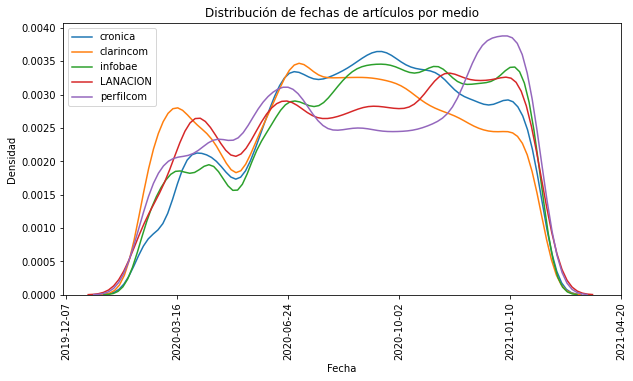
\includegraphics[width=\textwidth]{img/fechas_por_medios_todas.png}
    \caption{Distribución temporal de artículos recolectados}
    \label{fig:fecha_articulos_por_medio_todas}
\end{figure}



\begin{figure}
    \centering
    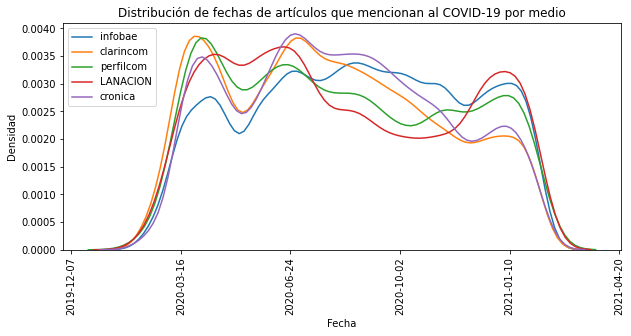
\includegraphics[width=\textwidth]{img/fechas_por_medios.png}
    \caption{Distribución temporal de artículos recolectados que mencionan COVID-19 o algún término relacionado}
    \label{fig:fecha_articulos_por_medio_covid}
\end{figure}



\section{Selección de datos a anotar}


Un problema que se nos presenta antes de comenzar el etiquetado es el de seleccionar los artículos que vamos a etiquetar. Una primera posibilidad para hacer esto es realizar una selección aleatoria de artículos y comentarios; sin embargo, los comentarios discriminatorios no se distribuyen de manera uniforme entre los artículos, sino que se concentra en algunos temas. Es mucho más probable encontrar comentarios de índole discriminatoria en notas que tengan temas cercanos a alguna de las características protegidas; por ejemplo, es esperable que encontremos contenido odioso en notas sobre China y el Coronavirus o sobre una chica transgénero antes que en un artículo de fútbol o economía. 


Teniendo esto en cuenta, evaluamos varias alternativas. La primera es observar los artículos e intentar seleccionar aquellos que consideremos que puedan tener contenido potencialmente discriminatorio. 

Una posibilidad para esto sería usar algunas palabras ``semilla'' para seleccionar artículos interesantes. Otra sería buscar directamente comentarios que contengan algunos insultos comunes o expresiones peyorativas hacia nuestros grupos protegidos. Después de algunos experimentos, decidimos utilizar el muestreo basado en comentarios.

\subsection{Selección en base a artículos}

En primer lugar, consideramos la posibilidad de hacer una selección en base al contenido de los artículos. Luego de realizar algunos experimentos usando LDA \cite{blei2003latent} para buscar tópicos posibles de las notas, decidimos realizar una selección un poco más controlada y determinística en base a la utilización de palabras clave. Es decir, seleccionaremos artículos en base a la aparición o no de ciertas ``semillas''

Para ello, indexamos todos nuestros artículos en MongoDB \footnote{\url{https://www.mongodb.com/}}, una base de datos no relacional y desestructurada. MongoDB permite la utilización de índices en base a texto, y realizar búsquedas en base a textos, palabras, e inflexiones. Cada artículo fue indexado en base al contenido de su cuerpo (es decir, el texto en sí del artículo).

La tabla \ref{tab:palabras_articulos} muestra el conjunto utilizado para recolectar artículos. Como vemos, hay diversas palabras que recogen distintas temáticas de posibles tópicos ``calientes'', algunos muy locales respecto a eventos concretos durante la pandemia. 

\begin{table}[]
    \centering
    \begin{tabular}{l | l | l | l}
    China        &  piqueteros              &  mamá                & empleadas domésticas  \\ 
    Cuba         &  villas                  &  de género           & la modelo             \\               
    cubano       &  la villa                &  aborto              & la periodista         \\            
    bolivia      &  movimientos sociales    &  actriz              & la cantante           \\               
    paraguayo    &  organizaciones sociales &  actrices            & travesti              \\               
    judío        &  tomas de tierras        &  feminista           & trans                 \\                 
    camionero    &  toma de tierras         &  femicidio           & gay                   \\               
    ladrón       &  sindicatos              &  enfermera           & homosexual            \\                 
    represión    &  Guernica                &  madre               & de la V               \\           
    criminal     &  mapuches                &  personal doméstico  & Ofelia                \\                      
    \end{tabular}
    \caption{Palabras utilizad}
    \label{tab:palabras_articulos}
\end{table}

\subsection{Selección en base a comentarios}

Otra posibilidad es mirar los comentarios de los artículos en lugar del contenido del artículo, y seleccionar posibles temas en base a esto. En este punto, la idea es únicamente seleccionar los artículos y no los comentarios; estos últimos son sólo usados como indicios para ver comentarios con posible contenido discriminatorio, y como tal identificar a ese artículo como un posible generador de este tipo de contenido. 

La idea es similar a la de la selección con artículos, sólo que aplicada a comentarios: buscamos comentarios que contengan alguna de las palabras semilla listadas en la Tabla \ref{tab:palabras_comentarios}. Estas palabras fueron recolectadas a base de experimentación y observación de los datos, y tratan de contener 

Una idea también considerada fue la de utilizar un clasificador entrenado sobre otro dataset (por ejemplo, el de \citet{hateval2019semeval}) y con eso marcar comentarios posiblemente discriminatorios. Sin embargo, muy probablemente detectaríamos sólo comentarios para las categorías/características etiquetadas en esos datasets e ignorarían las que agregamos en nuestro trabajo; por ejemplo, la mayoría de los datasets no contienen comentarios anotados contra la comunidad LGBTI.

El procedimiento de selección consta de, dado un artículo, marcar sus comentarios que contengan una o más de las expresiones listadas. Si el artículo tiene tres o más comentarios marcados, entonces seleccionamos el artículo; caso contrario, es descartado. 

Vale remarcar que este proceso de selección es para los \emph{artículos}, no para los comentarios.




\begin{table*}[t!]
    \centering
    \begin{tabular}{l|l|l|l|l|l|l}
    bija          & urraca     & viejo puto    & trolo      & peruano  & matarlos         & negra      \\
    prostituta    & tucán      & trabuco       & sodomita   & peruca   & una bomba        & negro de   \\
    feministas    & putita     & travesti      & chinos de  & judío    & vayan a laburar  & negros     \\
    feminazis     & reventada  & trava         & bolita     & sionista & vayan a trabajar & bala       \\
    aborteras     & marica     & degenerado    & paraguayo  & villeros & gorda            & uno menos  \\
    \end{tabular}
    \caption{Palabras utilizadas para recolectar comentarios}
    \label{tab:palabras_comentarios}
\end{table*}



Luego de algunos análisis experimentales y observacionales de las dos posibles metodologías, decidimos utilizar el muestreo de artículos en base a comentarios. Por lo que pudimos observar, los artículos seleccionados parecían tener mayor incidencia de mensajes odiosos y eso nos decantó hacia esa opción. 

\section{Criterios de anotación}
\label{sec:criterios}

La definición de lenguaje discriminatorio utilizada en este trabajo está basada en trabajos de la Comisión Interamericana de Derechos Humanos (CIDH)\cite{CIDH2015}, del Centro de Estudios de Libertad de Expresión (CELE) \cite{cele2019} y en el Article 19 Hate Speech Toolkit \cite{article192015}. 

Teniendo estos insumos en cuenta, entendemos que hay discurso discriminatorio en un texto social si contiene declaraciones de carácter intenso y posiblemente irracional de rechazo, enemistad y aborrecimiento contra un individuo o contra un grupo, siendo estos objetivos de estas expresiones por poseer (o aparentar poseer) una característica protegida.

Las características en cuestión son protegidas por leyes internacionales. En este trabajo consideramos las siguientes:

\begin{enumerate}
\item Sexo (Mujeres, concretamente)
\item Género o identidad sexual (Colectivo LGBTI)
\item Ser inmigrantes, extranjeros, pueblos aborígenes u otras nacionalidades (xenofobia, racismo)
\item Situación socioeconómica o barrio de residencia
\item Poseer discapacidades, problemas salud mental o de adicción al alcohol, drogas u otros estupefacientes
\item Opinión o ideología política
\item Aspecto o edad (mayormente, gordofobia/gerontofobia)
\item Antecedentes penales o estar privado de la libertad
\end{enumerate}

Si bien algunas de estas características no son consideradas en algunos tratados (por ejemplo, contra los presos), las tuvimos en cuenta por las características propias del tratamiento en medios durante la pandemia de distintos sucesos.


\section{Modelo de etiquetado}

Un modelo de anotación es, según \citet{pustejovsky2012natural}, una representación práctica del objetivo de anotación. En nuestro caso, queremos marcar comentarios discriminatorios, marcar a qué grupos y/o características se está ofendiendo, y también identificar llamados a tomar alguna acción contra los objetos de esos discursos. Por lo pronto, haremos una definición que capture ese objetivo sin deternos demasiado en especificarlo formalmente (lo que llaman en ese libro ``especificación''). 

\subsection{Modelo Jerárquico de Etiquetado}
\citet{zampieri2019predicting} introdujeron un modelo jerárquico de anotación para la tarea de lenguaje ofensivo, utilizado en las competiciones OffensEval \cite{zampieri2019semeval2019} y hatEval \cite{hateval2019semeval}. La idea de la anotación jerárquica es realizar anotaciones adicionales sólo para algunos casos de anotaciones del nivel anterior. 

En el caso de \emph{HatEval}, tenemos un primer nivel que consta de anotar si un tweet contiene o no lenguaje de odio (nivel 1). Si el tweet tiene lenguaje de odio, entonces anotamos si está dirigido a un individuo o a un grupo, y también anotamos si es agresivo o no (ambos nivel 2). En el caso de \emph{OffensEval}, primero anotamos si es ofensivo (nivel 1), luego si está dirigido o es un insulto no dirigido (nivel 2) y finalmente, si es dirigido y ofensivo, marcamos su objetivo (nivel 3). En la figura \ref{fig:modelos_offenseval_hateval} ilustramos ambos modelos. 


%
%
% Link: https://docs.google.com/drawings/d/1ZgTmvRwMWn0B-kokfw87jfSa7eY5-OSBHwltetnNT08/edit
%
 \begin{figure}
     \centering
     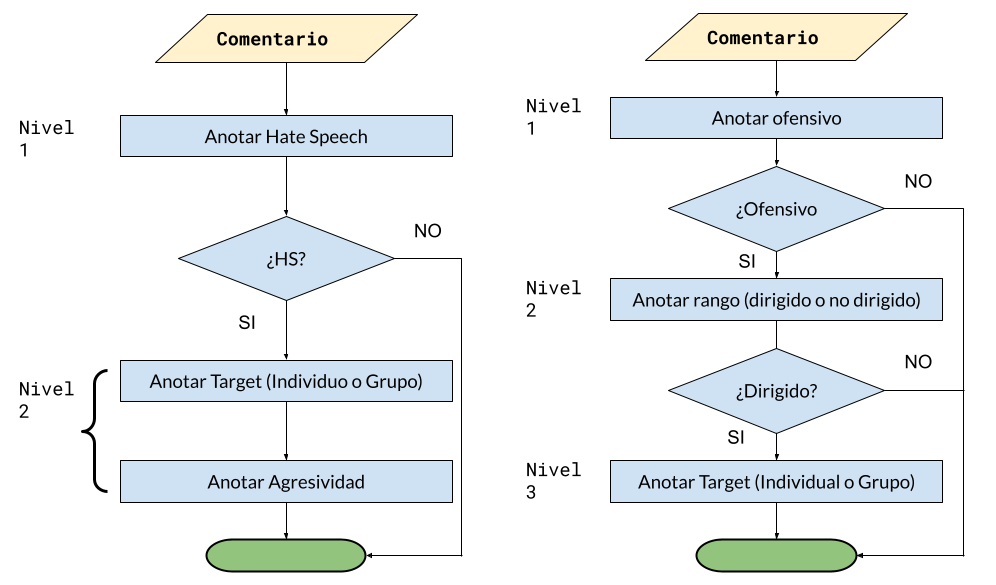
\includegraphics[width=\textwidth]{img/modelosjerarquicos.png}
     \caption{Modelos jerárquicos de anotación. A la izquierda, tenemos el modelo jerárquico propuesto para HatEval \cite{hateval2019semeval}, a la derecha el modelo propuesto para OffensEval \cite{zampieri2019semeval2019}}
     \label{fig:modelos_offenseval_hateval}
 \end{figure}

\subsection{Modelo de etiquetado jerárquico y contextualizado}



\begin{figure}
    \centering
    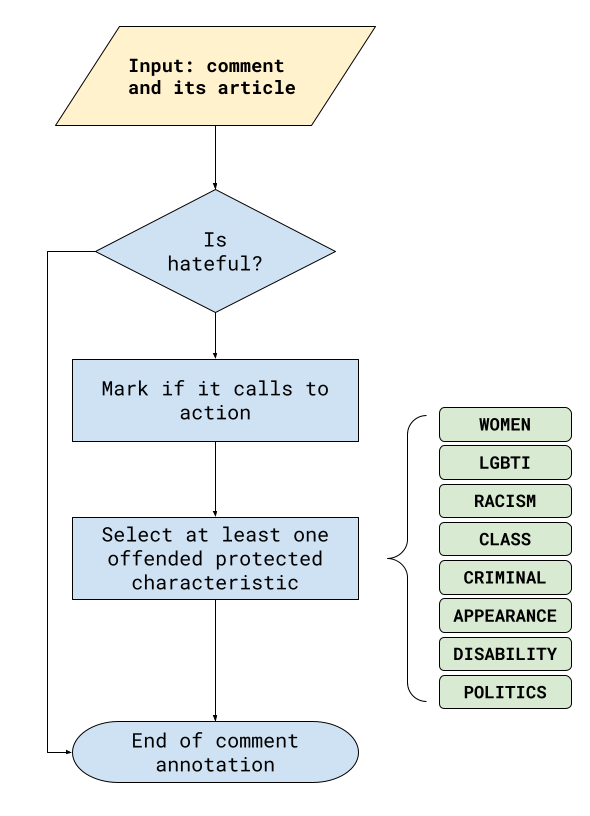
\includegraphics[width=0.70\textwidth]{img/Annotation Model.png}
    \caption{Modelo de anotación}
    \label{fig:annotation_model}
\end{figure}


La figura \ref{fig:annotation_model} muestra el modelo de anotación utilizado. Seguimos un modelo jerárquico similar al propuesto por \citet{zampieri2019predicting}, aunque de sólo un nivel. Para cada comentario y su respectivo contexto (el artículo), requerimos una anotación  para decidir si el comentario es odioso o no. Si no es odioso, no se necesita más información. Si es así, el par artículo-comentario debe contener, además, una anotación por si llama o no a la acción, y al menos una categoría protegida 




\section{Herramienta de etiquetado}

\section{Etiquetadores}

A diferencia de otros trabajos (como hatEval \cite{hateval2019semeval}), decidimos por un lado, garantizar que nuestros anotadores estén más cercanos culturalmente al problema en cuestión, a la vez que tener mayor control del perfil de estos. Consideramos que el discurso de odio tiene un fuerte componente cultural, muchas veces expresado a través de jerga o expresiones dialectales muy particulares, y relacionado con noticias muy propias de esta región.


\subsection{Tipos de anotación en otros trabajos}

Comentar otros trabajos acá

\begin{itemize}
    \item Davidson
    \item Waseem
    \item hatEval
    \item CONAN
    \item Gao (contextualizado)
    \item Context offensive (el de Google, y el griego)
\end{itemize}

\subsection{Perfil de etiquetadores}

Para la selección de anotadores, realizamos una búsqueda interna. Puntualmente, buscamos:

\begin{itemize}
    \item Estudiantes/graduades de carreras de Cs. Sociales, Psicología, Letras o afines
    \item Hablantes nativos (o casi) de Español Rioplatense
    \item Usuarios de redes sociales; preferentemente Twitter
\end{itemize}

Luego de una breve entrevista donde les contamos el proyecto y corroboramos que efectivamente sean hablantes nativos de Español Rioplatense y usuarios de RRSS, les mandamos una pequeña evaluación paga que constó de leer el manual de criterios de anotación (que agregamos en \ref{app:manual_criterios_anotacion}) y anotar 5 artículos. Esto lo realizamos para ver que efectivamente estén entendiendo la tarea. Estos artículos fueron luego reutilizados para el proceso de entrenamiento.

\section{Proceso de etiquetado}

\subsection{Preprocesado de los datos}

\subsection{Entrenamiento de etiquetadores}
\subsection{Esquema de anotación}
Acá anotar los 3 anotados, etc

%
% Esto quizás va después
%

\section{Dataset resultante}
\subsection{Estadísticas}
\subsection{Asignación}
\subsection{Agreements}
\subsection{Recursos utilizados}
\subsection{Anonimización para publicación de los datos}


\chapter{Proceso y resultados}
\chapter{Clasificadores, Análisis y Limitaciones}
\chapter{Conclusiones}


\appendix

% Manual de anotación

\chapter{Discurso de odio}
\label{app:04}

\section{Tratados internacional sobre libertad de expresión y discurso de odio}
\label{app:tratados-internacionales}

\subsection{Libertad de expresión}

La Convención Americana de Derechos Humanos (CADH) establece que:

\begin{displayquote}[CADH, Artículo 13][]

    1. Toda persona tiene derecho a la libertad de pensamiento y de expresión.  Este derecho comprende la libertad de buscar, recibir y difundir informaciones e ideas de toda índole, sin consideración de fronteras, ya sea oralmente, por escrito o en forma impresa o artística, o por cualquier otro procedimiento de su elección.

    2. El ejercicio del derecho previsto en el inciso precedente no puede estar sujeto a previa censura sino a responsabilidades ulteriores, las que deben estar expresamente fijadas por la ley y ser necesarias para asegurar:

    a)  el respeto a los derechos o a la reputación de los demás, o

    b) la protección de la seguridad nacional, el orden público o la salud o la moral públicas.
\end{displayquote}

En Estados Unidos, la primer enmienda protege este derecho humano, mientras que en la Unión Europea, legislación similar ofrece protección a la libertad de expresión. Finalmente, la declaración universal de los derechos humanos de la ONU \footnote{\url{https://www.un.org/es/about-us/universal-declaration-of-human-rights}} menciona tanto en su preámbulo como en el artículo 19

\begin{displayquote}[Declaración Universal de los Derechos Humanos][ONU]
    Todo individuo tiene derecho a la libertad de opinión y de expresión; este derecho incluye el de no ser molestado a causa de sus opiniones, el de investigar y recibir informaciones y opiniones, y el de difundirlas, sin limitación de fronteras, por cualquier medio de expresión.
\end{displayquote}


Otro documento conocido como el Pacto Internacional de Derechos Civiles y Políticos (ICCPR por sus siglas en inglés), sancionado en 1966 en la Asamblea de las Naciones Unidas y ratificado por 166 países, incluye en su artículo 19:

\begin{displayquote}[Artículo 19 de la ICCPR]
1. Nadie podrá ser molestado a causa de sus opiniones.

2. Toda persona tiene derecho a la libertad de expresión; este derecho comprende la libertad de buscar, recibir y difundir informaciones e ideas de toda índole, sin consideración de fronteras, ya sea oralmente, por escrito o en forma impresa o artística, o por cualquier otro procedimiento de su elección.

3. El ejercicio del derecho previsto en el párrafo 2 de este artículo entraña deberes y responsabilidades especiales. Por consiguiente, puede estar sujeto a ciertas restricciones, que deberán, sin embargo, estar expresamente fijadas por la ley y ser necesarias para:

a) Asegurar el respeto a los derechos o a la reputación de los demás;

b) La protección de la seguridad nacional, el orden público o la salud o la moral públicas.
\end{displayquote}


Este último apartado ilustra que la libertad de expresión no es un derecho completamente irrestricto. El ejercicio de los derechos e igualdad ante la ley de otros marca este límite. Citando nuevamente al Pacto de San José de Costa Rica:

\begin{displayquote}[Pacto San José de Costa Rica, CADH][Artículo 1]
    1. Los Estados Partes en esta Convención se comprometen a respetar los derechos y libertades reconocidos en ella y a garantizar su libre y pleno ejercicio a toda persona que esté sujeta a su jurisdicción, sin discriminación alguna por motivos de raza, color, sexo, idioma, religión, opiniones políticas o de cualquier otra índole, origen nacional o social, posición económica, nacimiento o cualquier otra condición social.
\end{displayquote}

y a la Declaración Universal de los Derechos Humanos de la ONU:

\begin{displayquote}
    Todos los seres humanos nacen libres e iguales en dignidad y derechos y, dotados como están de razón y conciencia, deben comportarse fraternalmente los unos con los otros.
\end{displayquote}


\subsection{Discurso de odio}

Una recopilación de definiciones realizada por un informe de la UNESCO

\begin{displayquote}[Countering Hate Speech Online, \citet{gagliardone2015countering}]
    Mientras que el sistema interamericano de derechos humanos ha desarollado determinados estándares, no existe una definición universalmente aceptada de “discurso de odio” en el derecho internacional. Según un reciente informe emitido por la UNESCO que estudió las distintas definiciones de discurso de odio en el derecho internacional, el concepto con frecuencia se refiere a “expresiones a favor de la incitación a hacer daño (particularmente a la discriminación, hostilidad o violencia) con base en la identificación de la víctima como perteneciente a determinado grupo social o demográfico. Puede incluir, entre otros, discursos que incitan, amenazan o motivan a cometer actos de violencia. No obstante, para algunos el concepto se extiende también a las expresiones que alimentan un ambiente de prejuicio e intolerancia en el entendido de que tal ambiente puede incentivar la discriminación, hostilidad y ataques violentos dirigidos a ciertas personas
\end{displayquote}



\chapter{Construcción de dataset contextualizado de discurso de odio}
\label{app:05}
\chapter{Apéndice: Construcción de dataset contextualizado de discurso de odio}
\label{app:02}

En este apéndice describiremos algunos pormenores de la construcción del dataset descripta en el capítulo \ref{chap:05_dataset_creation}.




\section{Distribución de datos recolectados}
\label{app:distribucion_datos}
La figura \ref{fig:fecha_articulos_por_medio_todas} muestra la distribución temporal de los artículos, sin aplicar ningún filtro por palabras, mientras que \ref{fig:fecha_articulos_por_medio_covid} muestra aquellas relacionadas al COVID-19 utilizando el filtro de palabras listado en la tabla \ref{tab:article_words}. Podemos observar dos caídas. Hay un pequeño pozo en mayo 2020 que se debió a la caída de nuestros servidores de recolección. Por otro lado, observamos que algunos medios (particularmente La Nación) parecieran mencionar menos directamente al COVID (al menos con los términos referidos anteriormente) hasta un nuevo pico cerca de fin de año, coincidente con un nuevo rebrote del virus en este país.

Sin embargo, todo esto puede ser un artefacto del método de filtrado: muchas notas contienen links a otras con sus títulos y eso puede interferir en estas estimaciones. Así y todo, decidimos mantener este método ya que consideramos que mayormente las notas en el período referido tienen relación con la pandemia.


\begin{figure}
    \centering
    \begin{subfigure}[t]{\textwidth}
        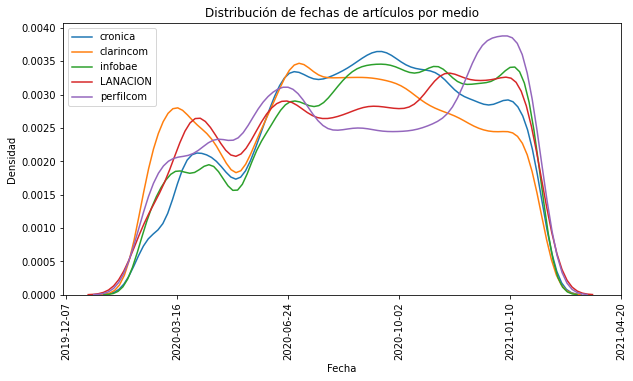
\includegraphics[width=\textwidth]{img/fechas_por_medios_todas.png}
        \caption{Distribución temporal de artículos recolectados, sin aplicar ningún filtro}
        \label{fig:fecha_articulos_por_medio_todas}
    \end{subfigure}

    \begin{subfigure}[t]{\textwidth}
        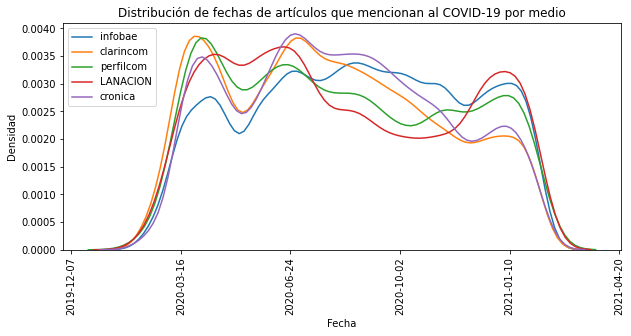
\includegraphics[width=\textwidth]{img/fechas_por_medios.png}
        \caption{Distribución temporal de artículos recolectados que mencionan COVID-19 o algún término relacionado}
        \label{fig:fecha_articulos_por_medio_covid}
    \end{subfigure}

    \caption{Gráficos de distribución de los datos recolectados. La figura \ref{fig:fecha_articulos_por_medio_todas}}
\end{figure}


\section{Recursos utilizados}

El etiquetado constó de XXX horas. A cada etiquetador le fue pagado YYYY por hora, y luego ZZZ por hora en segunda instancia. Esto equivale a WWW USD.

\section{Manual de criterios de anotación}
\label{app:manual_criterios_anotacion}
\chapter{Manual de criterios de anotación}
\label{app:manual_criterios_anotacion}
\section{Presencia de lenguaje discriminatorio}

Entendemos que hay discurso discriminatorio en el tweet si contiene declaraciones de carácter intenso y posiblemente irracional de rechazo, enemistad y aborrecimiento contra un individuo o contra un grupo, siendo estos objetivos de estas expresiones por poseer (o aparentar poseer) una característica protegida.

Este discurso puede manifestarse de manera explícita (insultos directos), celebraciones sobre asesinatos u otros crímenes, o bien otras expresiones más veladas. Lo que queremos captar es la intención del autor del tweet. El carácter discriminatorio de un mensaje está dado tanto por el contexto (en este caso, el tweet original del medio periodístico y posiblemente la nota) y el contenido del tweet en sí mismo. Por ejemplo, un comentario que diga “excelente” sin contexto es una cosa, y decir eso mismo en una nota que relata un femicidio, o un asesinato es otra muy distinta.

Las características protegidas que vamos a tener en cuenta son las siguientes:

\begin{enumerate}
\item Sexo (Mujeres, concretamente)
\item Género o identidad sexual (Colectivo LGBTI)
\item Ser inmigrantes, extranjeros, pueblos aborígenes u otras nacionalidades (Xenofobia, racismo)
\item Situación socioeconómica o por barrio de residencia
\item Poseer discapacidades, problemas salud mental o de adicción al alcohol u otros estupefacientes
\item Opinión o ideología política
\item Aspecto o edad (mayormente, gordofobia/gerontofobia)
\item Antecedentes penales o estar privado de la libertad

\end{enumerate}

Es decir, para considerar un mensaje como discriminatorio, debe cumplir que el discurso discriminatorio está orientado hacia un individuo o grupo de al menos una (aunque posiblemente más de una) característica protegida.


Consideramos que el mensaje del tweet (a la vez que el receptor del odio) es el que determina si puede o no ser considerado discriminatorio y hacia qué grupo está dirigido. Esto puede no necesariamente coincidir con el destinatario explícito del mensaje: por ejemplo, si alguien le dice a Susana Giménez “judía sionista hdp”, a pesar de no ser Susana Giménez judía, se puede considerar esto como discurso de odio contra las minorías religiosas y/o discurso xenófobo.


\section{Llamado a la acción}

Entendemos que un tweet (que contiene discurso discriminatorio) llama a la acción si contiene alguna incitación a tomar algún tipo de medida contra el sujeto o grupo ofendido. Esta medida puede ser de carácter violento (“hay que matarlos ya” “pongámosles una bomba”) o de carácter menos violento (“hay que dejar de comprarles a estos chinos ladrones”)

Estos tweets nos interesan particularmente porque son los más peligrosos y dañinos: los que llaman a tomar algún tipo de represalia contra la persona o el grupo en cuestión.

\section{Características protegidas}

Finalmente, para cada tweet deberemos marcar qué grupo o característica protegida es atacado. En este caso, necesariamente un grupo/característica debe ser seleccionado:

Usaremos una notación abreviada en la interfaz de etiquetado, en la que algunos de los grupos o características mencionadas fueron reagrupadas de la siguiente manera:

\begin{enumerate}
    \item MUJER: por su sexo
    \item LGBTI: por género o identidad sexual
    \item RACISMO: Por ser inmigrantes, extranjeros, pueblos aborígenes u otras nacionalidades (Xenofobia, racismo)
    \item POBREZA: Por situación socioeconómica o por barrio de residencia.
    \item DISCAPAC: Por tener discapacidades, problemas salud mental o de adicciones
    \item POLITICA: Por su opinión o ideología política
    \item ASPECTO: Por su aspecto o edad
    \item CRIMINAL: Por sus antecedentes o situación penal (presos)
\end{enumerate}

A su vez, agregamos la categoría “OTROS”. Esta categoría es excepcional, y debería utilizarse sólo si algún tipo de discriminación no está contemplado en estas categorías.

Respecto a la discriminación de carácter político tiene que ser algo más que una mera opinión  sino tener una componente irracional, de descalificación y de aborrecimiento considerable sobre un individuo o una facción política.

No se contempla dentro de las categorías protegidas a las profesiones. Es decir, no tenemos en cuenta el discurso contra científicos, médicos, o periodistas; de esto último hay bastante material agresivo en los comentarios.


\subsection{Lineamientos generales}

El discurso discriminatorio no es sólo discurso ofensivo contra una persona o grupo con alguna de las características protegidas. Tiene que apelar a su condición de mujer, inmigrante, LGBTI, etc. para que lo consideremos así.

Por ejemplo: si alguien agrede a una mujer, a un inmigrante, o a alguien de la comunidad LGBTI, no necesariamente está incurriendo en un discurso discriminatorio salvo que apele a algo que remita a su característica como tal.


Expresiones de aprobación ante noticias de crímenes o acciones contra persona o grupo de las características protegidas son consideradas discriminatorias.

\subsubsection{Ejemplos}

Violan a la reconocida actriz XXXX YYYY
Asesinan a un comerciante chino por creer que tenía Coronavirus
Motín y muerte en la prisión de Marcos Paz

Comentarios de contenido discriminatorio: (emoji de aplausos) - uno menos - bravo! -


Si no queda claro que haya un mensaje discriminatorio o parece de carácter difuso o demasiado tangencial, entonces etiquetar como no discriminatorio




\subsection{MUJER}

Insultar a una mujer sin hacer ninguna referencia particular a su condición de mujer no es suficiente para ser considerado discurso discriminatorio

Como regla: si el mismo insulto o agresión aplicase contra un hombre, entonces no debiéramos considerarlo como discriminación


Insultos contra las expresiones políticas del movimiento de las mujeres son consideradas en esta categoría: si se las insulta como feminazis, aborteras, pañuelito verde, etc



Apelaciones a su apariencia o aspecto propias de una mujer son consideradas en esta categoría. En este punto consideramos comentarios cosificadores


Insultar como “vieja” a una persona no califica como misoginia. Usar para ese caso la categoría ASPECTO que contempla la gerontofobia

EJEMPLOS:

Nati Jota furiosa por los comentarios que recibe en las redes.

Comentarios sexistas:

Pero si sos de plástico nena! (opina de manera denigratoria de su apariencia)
Flor de gato!
Miauuu!
A esta sólo se la conoce por su cuerpo y ahora se hace la santa. Andá a estudiar
Le damos hasta que San Lorenzo vuelva a Boedo
Y esta rubia tarada quién es?



Comentarios ofensivos pero no sexistas:
Callate forra (ofensivo pero no particularmente sexista)
Y esta quién es? A quién le importa?
Quién?
Nati cuánto?
Esta también recibe sobres?
Otra descerebrada más (súper agresivo, pero es un comentario que podría recibir un hombre, aunque en menor cantidad…)
Andá a cagar..boluda..conductora de 4ta..
HDP
Boba



\subsection{LGBTI}

Expresiones de disgusto o rechazo del estilo “qué asco” frente a integrantes de la colectividad deben ser marcados como discurso discriminatorio


Apelaciones a la anatomía o del estilo “biologicistas” deben ser marcados como discurso discriminatorio


Ejemplos:

Anibal Pachano sobre la cuarentena: “este virus nos está destruyendo a los actores”


Comentarios discriminatorios:

Qué asco este sujeto
Y a este trolo quién le pidió su opinión?
Me desagrada


Comentarios ofensivos pero no discriminatorios:

Ajá, y?
No me importa tu opinión, gracias
Se acuerdan cuando este atacaba a Cristina? Andá a llorarle al gato, Aníbal
Pelotudazo!


Famosa actriz trans dio una entrevista a La NACION: “Como mujer, estoy en la mejor etapa de mi vida”


Comentarios discriminatorios:

Muy lindo todo, pero sos hombre
“Mujer” dice jajajaj naciste y morirás macho
Qué asco este trolo
(emoji de asco)
Una mujer con sorpresa
Trava horrendo
Perdón pero qué nombre dice tu DNI?


Comentarios ofensivos pero no discriminatorios:

Quién?
Y a quién le interesa lo que diga esta mujer?
Que se vaya a cagar
Agradecele al gobierno de Néstor que tenés derechos





\subsection{RACISMO}

Asignar a todo un pueblo con una característica o actividad particular negativa entra en esta categoría
Cualquier llamada a expulsar, matar, tirar bombas, destruir, aniquilar, etc a un pueblo, inmigrantes o país entra en esta categoría. Más aún, deben ser marcadas como “llamadas a la acción”
Teorías conspirativas (hasta cierto punto) o acusaciones a un Gobierno/Estado no deberían entrar en esta categoría
¿Acusaciones respecto al virus?



Ejemplos:

Rescatan en China a cuarenta gatitos bebé que iban a ser utilizados en restaurantes


Comentarios discriminatorios:

Chinos asquerosos
Malparidos! Chinos de mierda
Sigan desparramando pestes hijos de puta!
Por qué no se comen entre ellos?
País horrible y enfermo
Estos chinos nos diseminan su peste por todo el mundo

Comentarios discriminatorios y que además llaman a la acción:

Son una plaga estos chinos, hay que matarlos a todos
Ojalá les caigan veinte bombas
Hay que barrer ese país de la faz de la tierra

Comentarios ofensivos pero no racistas:

Son comunistas, qué querés
Lo rescataron a Mauri?




Otros comentarios no racistas

El gobierno chino está intentando controlar todo, cuidado
Mienten con que controlaron el virus, cómo no van a mentir con esto también?
De terror!


Tomas de terrenos: se profundizan las tomas en todo Buenos Aires


Comentarios discriminatorios:

Rajen a todos los peruanos de las tomas! (llama a la acción, además)
Increíble, cualquier paraguayo o bolita de mierda te saca la casa

\subsection{POBREZA}

Expresiones denigrantes sobre la condición socioeconómica son consideradas discriminatorias: referirse a las personas sin empleo como “vagos”, a otros como “(chori)planeros”
Respecto a la gente que posee planes de asistencia social, si es una opinión general sin ser ofensiva no se considera discriminatoria (del estilo “hay que reducir el gasto social y los planes”, “perdieron la cultura del trabajo”)

Presupuesto: aumentó el gasto en planes asistenciales durante la pandemia

Ejemplos discriminatorios:

Basta de mantener vagos!
Cansada de los planeros
Che laburar estos atorrantes ni en pedo no?
PARASITOS

Ejemplos no discriminatorios

La gente que trabaja y aporta impuestos es cada vez menos. Estamos al horno



\subsection{POLITICA}

Apreciaciones derogatorias sobre la posición política son consideradas discriminatorias : zurdo/a, bolchevique, peroncho, gorila, kuka, etc
Acusaciones de corrupción o de “recibir sobres” no son consideradas discriminatorias
Tampoco aquellas expresiones que traten de inútiles a funcionarios
Tratar de viejo/a, gordo/a, u otras cuestiones físicas deben ser marcados en las categorías respectivas, no acá

Aumentó el gasto en planes asistenciales durante la pandemia

Ejemplos discriminatorios:

BASTA ZURDOS DE ROBARNOS
Bolcheviques de mierda

Ejemplos no discriminatorios

La gente que trabaja y aporta impuestos es cada vez menos. Estamos al horno
Qué gobierno de inútiles
Son unos delincuentes
Hijos de mil puta!
Siguen volando los sobres para el Congreso
Siga siga la impresión




\subsection{ASPECTO}

Apreciaciones denigrantes sobre la apariencia de una persona y/o su edad
Principalmente, tenemos en mente la gordofobia y gerontofobia, pero puede referir a otras características físicas (por ejemplo, la altura)
En casos en las cuales haya solapamiento con mujer, marcar ambas


Luis Brandoni: “No convoqué el banderazo”

Ejemplos discriminatorios:

Viejo de mierda!
Qué decrépito impresentable que es este señor
Estás gagá, pelotudo

Jorge Lanata vuelve a la televisión

Ejemplos discriminatorios:

Gordo chanta otra vez volvés a vender pescado podrido?
porque no te vas vos tambien con todos bola de sebo!!!1
Estás gagá, pelotudo









\subsection{CRIMINAL}

Cualquier comentario que celebre acciones contra criminales o personas privadas de su libertad (golpizas, asesinatos, muerte en motines, etc) entra en esta categoría
En este ítem muchas veces veremos que son llamados a la acción: el de “matarlos”, llamar a reducir sus derechos, etc
Muere un delincuente tras un enfrentamiento con la policía

Ejemplos discriminatorios:

Uno menos!
Excelente!
(emoji de aplausos)
Que pena, pobrecito

Ejemplos que además llaman a la acción

MUY BIEN! Felicitaciones al policía, hay que liquidarlos sin piedad


1...100 101..200 …. 501...600

Primera fase: Et 1 => 1..100, Et 2 => 101 .. 200 … Et 6 => 501..600
Segunda fase Et2 => 1..100 Et1 => 101..200…. Et 6 => 401..500 Et 5 => 501..600

Shufflear temporalmente

Ejemplos no discriminatorios


Cómo puede ser que nuestra Ministra no haga nada?
La policía actuó correctamente.

Motín por el Coronavirus en Olmos: 3 muertos

Ejemplos discriminatorios y que llaman a la acción

Hay que rociar con nafta todas las cárceles
Soltemos 3 o 4 infectados con COVID en cada cárcel y problema solucionado
Paredón y listo



\subsection{DISCAPACIDAD}

Referencias peyorativas de adicciones a drogas, alcohol u otros estupefacientes
También referencias peyorativas a la salud mental de la persona en cuestión
Decir “está loco” no entra acá :-)
Malena Pichot sale a cruzar a Baby Etchecopar
Ejemplos discriminatorios:

Callate faloperita!
Jorge Lanata vuelve a la televisión

Ejemplos discriminatorios:

Che no probaste dejar la merca gordo?

Noticia sobre Patricia Bullrich...

Ejemplos discriminatorios:

Largá la (emoji de botella) Pato
Borracha hdp



\subsection{OTROS}

Esta categoría está reservada para cualquier otro tipo de discriminación que no esté contemplada en las categorías mencionadas
Insultos a profesiones (científicos, periodistas, por ejemplo) no entran en este apartado
ESTA CATEGORIA ES SUMAMENTE EXCEPCIONAL. NO USAR INDISCRIMINADAMENTE


\chapter{Apéndice Capítulo 6}
\label{app:06}

En este apéndice incluímos tablas y resultados completos


\section{Análisis comparativo entre clasificadores granulares y binarios}


\begin{table}[ht!]
    \centering
    \footnotesize
    \tbf{LGBTI}
    \begin{tabular}{p{0.03\textwidth} p{0.05\textwidth} p{0.45\textwidth} p{0.40\textwidth}}
        \hline
        1 & FN & Mara Gómez: la historia de la primera futbolista trans en el torneo argentino & Ponga huevos, Mara ponga huevos... \\
        2 & FN & Graciana Peñafort: "La marcha me dio mucha pena y tuvo un nivel de convocatoria menor al esperado" & Pena das vos, termotanque de lipídos y déficit fiscal \\
        3 & FP & "No soy feminista, soy mujer ", la frase de Viviana Canosa que generó polémica & La condición de mujer no la exime de ser una pelotuda y terrible hija de puta. Asi como tampoco la exime de vivir en un mundo con menos oportunidades, menores remuneraciones y más riesgos x el solo hecho de ser mujer, aunque no quiera luchar x eso. \\
        4 & FP & T ras una ráfaga de más de 20 disparos asesinaron a una mujer trans en Rosario & Con que le dispararon? Alta minigun tiene que ser para que 20 tiros sean solo una ráfaga y no una fullauteada \\
    \end{tabular}
    \tbf{RACISMO}
    \begin{tabular}{p{0.03\textwidth} p{0.05\textwidth} p{0.45\textwidth} p{0.40\textwidth}}
        1 & FN & Es hija de chinos, llevó merienda al colegio para compartir y se la rechazaron por temor a contagiarse de coronavirus &  Con lo hijos de puta, maleducados e intransigentes que son los chinos, si fuese al revés ya nos hubiesen embarcado a la estratosfera. Nadie ha visto como echan a los chicos pobres de los super por el miedo a que los afanen? Hablando de prejuicios \\
        1 & FN & Multitudes en las calles y discotecas abarrotadas: la fiesta de Wuhan tras el año de la pandemia que se inició en uno de sus "mercados húmedos" &  Los odio \\
        1 & FN & Su novia es mexicana y Migraciones le exige casi 50 mil pesos para dejarla ingresar a la Argentina &  Mira si le cobran eso a cada venezolano colombiano peruano chino boliviano que vienen al país a chupar sangre ,pagamos la deuda externa y nos volvemos potencia mundial \\
        1 & FP & URGENTE: Un hombre se incrustó con su auto en la puerta de la Embajada de China y aseguró que tenía explosivos & No es hombre . Es un boludo \\
        1 & FP & Su novia es mexicana y Migraciones le exige casi 50 mil pesos para dejarla ingresar a la Argentina &  Que me traiga una botellas de tequila del bueno \\
        1 & FP & El principal gremio docente nacional rechazó el regreso a las clases presenciales &Banda de VAGOS \\
        1 & FP & China: identificaron otro virus "con potencial para convertirse en pandemia" nuevo virus china transportado por cerdos podría infectar ahumanos las actuales vacunas podrían adaptarse más en la nota & PERO LA PUTA MADRE VIEJO \\
    \end{tabular}
    \caption{Ejemplos donde el clasificador granular acierta y el binario falla. FN marca que el clasificador binario no detecta el comentario como discriminatorio mientras que el contextualizado sí lo hace; FP es al revés, que el clasificador binario marca erróneamente el comentario como discriminatorio. Agrupadas de acuerdo a ciertas características; en el caso de los falsos positivos esta categoría es especulativa}
    \label{tab:fine_vs_plain_comparison}
\end{table}
% Capítulo 7 - Tablas de resultados de ajuste de dominio
\chapter{Adaptación de dominio}
\label{app:07}


En la tabla \ref{tab:full_domain_adaptation_evaluation_results} tenemos los resultados para todos los modelos considerados en el benchmark de adaptación de dominio, referidos en la sección \ref{sec:domain_adaptation_results}. Notamos, para compacidad, con subíndice \emph{U, C, D} a las versiones  \emph{uncased}, \emph{cased} y \emph{deacc}. Así mismo, notamos con $10K$ (por ejemplo) a aquel modelo con adaptación de dominio por 10,000 pasos según descripto en la sección \ref{sec:domain_adaptation_vs_robertuito}.

Podemos observar que, observando el score general, el mejor modelo adaptado a dominio para las versiones \emph{uncased} es beto$_{U10K}$, y para las versiones \emph{cased} es \beto{}$_{C5K}$; si bien en este último caso tiene una performance muy similar al de 20K pasos (de hecho, omitiendo la tarea de discurso de odio contextualizado gana por mínimo margen el de 20K).

\begin{sidewaystable}
    \centering
    \large
    \begin{tabular}{llllllr}
        \toprule
        Modelo             & CHATE                   &  HATE              &  SENTIMENT        &  EMOTION          &  IRONY            &     score \\
        \midrule
        beto$_{U5K}$   & $0.557 \pm 0.007$ & $0.756 \pm 0.012$ & $0.654 \pm 0.005$ & $0.509 \pm 0.014$ & $0.684 \pm 0.007$ &  0.632 \\
        beto$_U$        & $0.591 \pm 0.006$ & $0.757 \pm 0.012$ & $0.649 \pm 0.005$ & $0.521 \pm 0.006$ & $0.702 \pm 0.008$ &  0.644 \\
        bertin          & $0.557 \pm 0.008$ & $0.767 \pm 0.005$ & $0.665 \pm 0.003$ & $0.518 \pm 0.012$ & $0.716 \pm 0.008$ &  0.645 \\
        beto-cased      & $0.582 \pm 0.007$ & $0.768 \pm 0.012$ & $0.665 \pm 0.004$ & $0.521 \pm 0.012$ & $0.706 \pm 0.007$ &  0.648 \\
        roberta-bne     & $0.577 \pm 0.004$ & $0.766 \pm 0.015$ & $0.669 \pm 0.006$ & $0.533 \pm 0.011$ & $0.723 \pm 0.017$ &  0.653 \\
        beto$_{C2.5K}$  & $0.580 \pm 0.005$ & $0.771 \pm 0.007$ & $0.677 \pm 0.006$ & $0.525 \pm 0.010$ & $0.717 \pm 0.008$ &  0.654 \\
        beto$_{C10K}$   & $0.574 \pm 0.008$ & $0.782 \pm 0.009$ & $0.680 \pm 0.006$ & $0.524 \pm 0.006$ & $0.720 \pm 0.007$ &  0.656 \\
        beto$_{C20K}$   & $0.572 \pm 0.006$ & $0.777 \pm 0.009$ & $0.686 \pm 0.005$ & $0.517 \pm 0.009$ & $0.730 \pm 0.004$ &  0.656 \\
        beto$_{C5K}$    & $0.576 \pm 0.002$ & $0.781 \pm 0.010$ & $0.677 \pm 0.004$ & $0.525 \pm 0.016$ & $0.724 \pm 0.009$ &  0.657 \\
        beto$_{U20K}$   & $0.588 \pm 0.007$ & $0.768 \pm 0.012$ & $0.684 \pm 0.005$ & $0.533 \pm 0.016$ & $0.712 \pm 0.009$ &  0.657 \\
        beto$_{U2.5K}$  & $0.588 \pm 0.004$ & $0.784 \pm 0.011$ & $0.676 \pm 0.005$ & $0.533 \pm 0.008$ & $0.715 \pm 0.007$ &  0.659 \\
        beto$_{U10K}$   & $0.588 \pm 0.003$ & $0.775 \pm 0.015$ & $0.680 \pm 0.004$ & $0.553 \pm 0.009$ & $0.717 \pm 0.005$ &  0.663 \\
        robertuito$_C$  & $0.590 \pm 0.005$ & $0.790 \pm 0.012$ & $0.701 \pm 0.012$ & $0.519 \pm 0.032$ & $0.719 \pm 0.023$ &  0.664 \\
        robertuito$_{D}$& $0.593 \pm 0.006$ & $0.798 \pm 0.008$ & $0.702 \pm 0.004$ & $0.543 \pm 0.015$ & $0.740 \pm 0.006$ &  0.675 \\
        robertuito$_U$  & $0.593 \pm 0.004$ & $0.801 \pm 0.010$ & $0.707 \pm 0.004$ & $0.551 \pm 0.011$ & $0.736 \pm 0.008$ &  0.678 \\
        \bottomrule
    \end{tabular}
    \caption{Resultados de la evaluación de modelos pre-entrenados y modelos ajustados en dominio para el benchmark de tareas sociales: CHATE es contextualized hate speech, HATE es hate speech detection sobre el dataset de hatEval, SENTIMENT, EMOTION e IRONY son análisis de sentimiento, emociones e ironía sobre los corpus de TASS. Todos los scores son Macro F1s. beto-cased-ft y beto-uncased-ft son modelos adaptados al dominio sociall. Score es la media de cada fila. Gap es.. delta es...}

    \label{tab:full_domain_adaptation_evaluation_results}

\end{sidewaystable}





%%%% BIBLIOGRAFIA
\backmatter
\bibliography{biblio.bib}

\end{document}
